%\documentclass[aip, jcp, preprint]
\documentclass{article}[12pt]
\usepackage{graphicx}
\usepackage{amsmath}
\usepackage[margin=1in]{geometry}
\usepackage{color}

\title{Invite to Quote Rate Trends at Thumbtack}
\author{Ryan Applegate}
\begin{document}

\maketitle

\section{Data Exploration}

Trends and changes in the invite-to-quote rate at Thumbtack are explored
using linear fits on of binned time of invite data.

I construct the invite-to-quote data (hereafter "the data") by querying the
provided databases. Only the "requests" table contains valuable category and
location info and the quote response is found only in the "quotes" table. To
merge these essential fields into a single "invite" entity, I create a gathering
class "Invite" which houses all the fields necessary for downstream analysis. From
there, I query "invites", followed by "requests" and "quotes" and merge into a giant
list containing "Invite" objects. I am now in a position where I can tell you everything
about an invite, its location, category, the time it was sent, the originating request info
and if the invite received a response.

My analysis stack takes as input any list of Invites and builds a Pandas DataFrame,
performs a linear regression to find the trend in the invite-to-quote rate, and optionally
prints the fit/plot. Below is a plot where the data is binned daily. Understanding the plots
works as reading the percentage of invites that receive a response on the y-axis and the time
(in days or weeks of the year) on the x-axis. 

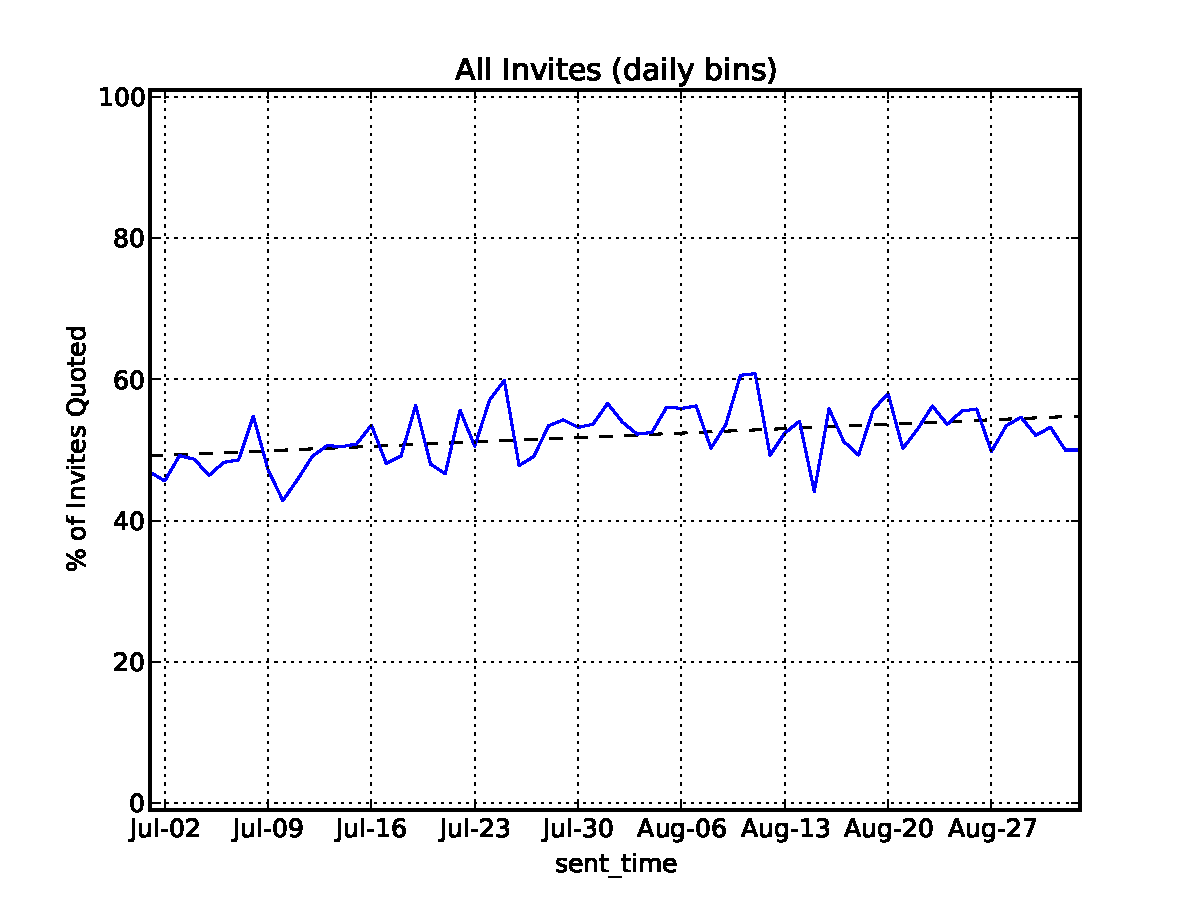
\includegraphics[scale=0.7]{../All_Invites_daily.pdf}

\noindent
Daily binning works by truncating the time portion of python datetime objects, grouping 
together all invites sent on the same calendar day. For all data, this works well and the fit is
significant, showing a growth in the invite-to-quote rate of $5.6\%$ over roughly two months.
The significance of the linear trend comes from a $pvalue_{all} = 0.00054$ which very strongly
rejects the null hypothesis that there is no trend in the data (that it's flat).

Very shortly, I will examine by location and by category invite lists which are much smaller datasets,
have more noise, and don't play as nicely with the daily binning scheme. To attempt to combat this, I 
create a weekly binning scheme which groups invites by the week of the year in which they occur. A
weekly binned trend line for all invite data is shown in the plot below.

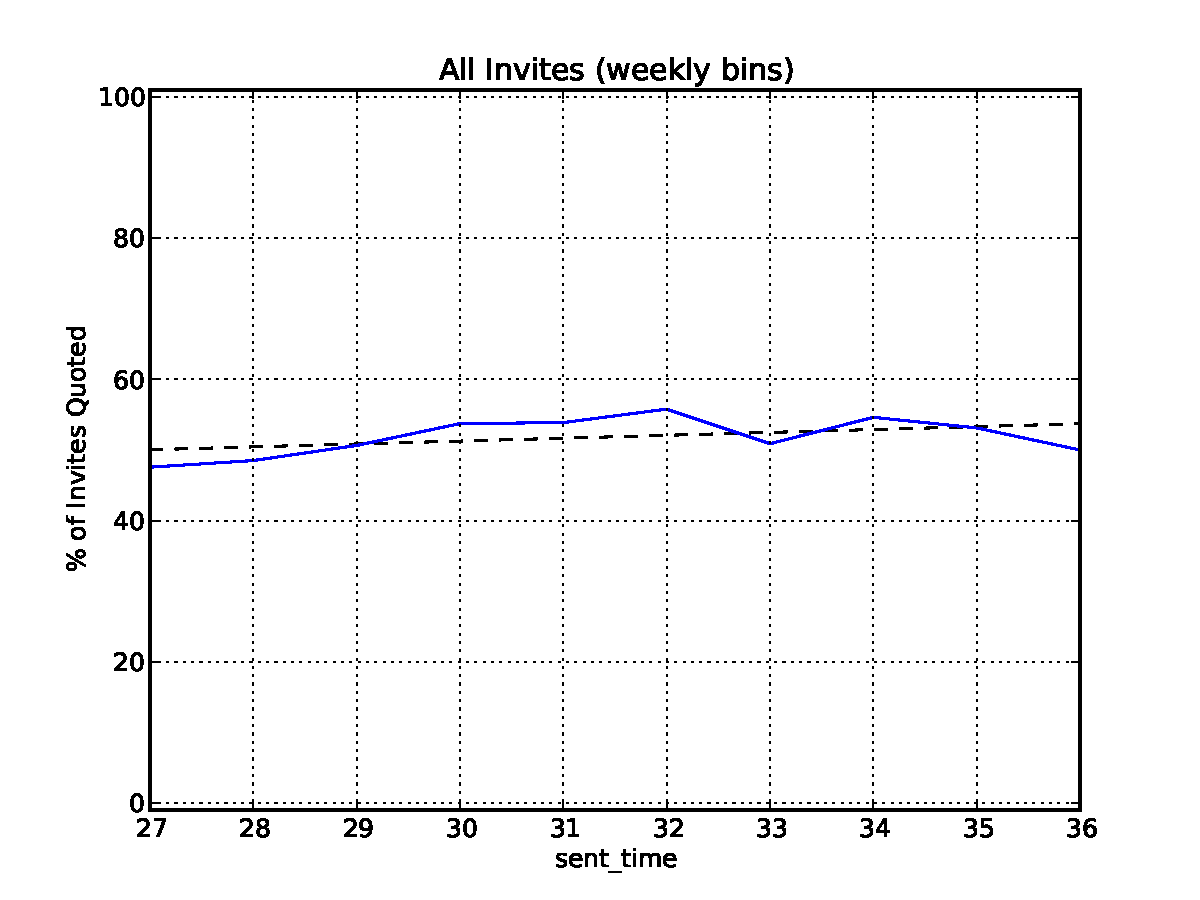
\includegraphics[scale=0.7]{../All_Invites_weekly.pdf}

In this situation, the growth of the invite-to-quote rate is $3.7\%$ with a $pvalue_{all} = 0.19$. So in fact, one can see here that binning too much has lowered the growth but more importantly given a less significant result. This illustrates the need to try different binning schemes for such data and carefully state results with respect to the binning you have done.

The code which builds dataframes and trend lines is attached and utilizes the functions
daily\_reponse\_dataframe and weekly\_response\_dataframe, daily\_trend\_line and weekly\_trend\_line,
daily\_quote\_growth and weekly\_quote\_growth, along with some helper functions to\_days and to\_weeks
for plotting and binning the invite sent times.


\section{Categories and Locations}

As different markets have highly varying factors determining service effectiveness, breaking
down the invites by market may provide important information for targeted product refinement.
In the data given, the category and location fields demand some attention and naturally fit into
the stack I have already built above. My stack takes any invite list as input and I can group all
invites by either category or location and process each group one at a time. This results in the same
dataframe, linear fit, growth change output as before, but now for a small segment of all data.

Grouping the invites is done by keying on the group\_id (category\_id or location\_id) which has
bene stored in the Invite class. A dictionary now exists that can be access by group and yields a
list of invites, precisely the input my analysis stack can already handle.

The by\_group() function takes a group dictionary and another dictionary which looksup actual
group names from group\_ids and iteratively runs my stack on each invite list.

\begin{verbatim}
def by_group(group_dict, groups):
    group_growth = {}
    for group_id in group_dict:
        df_daily = daily_response_dataframe(group_dict[group_id])

        daily_params = daily_trend_line(df_daily)
        print(groups[group_id], len(df_daily), daily_params[3])
        if daily_params[3] > 0.05 or len(df_daily) < 10:
            df_week = weekly_response_dataframe(group_dict[group_id])
            week_params = weekly_trend_line(df_week)
            print("\t", week_params[3])
            if week_params[3] > 0.05 or len(df_week) < 5:
                continue
            else:
                group_growth[group_id] = weekly_quote_growth(df_week, week_params)
        else:
            group_growth[group_id] = daily_quote_growth(df_daily, daily_params)

    group_list = [(groups[x], group_growth[x]) for x in group_growth]
    group_list.sort(key=lambda t: t[1])
    print(group_list)
\end{verbatim}

The flow of the above code is to attempt a daily binning and check the p-value, which is held in params[3]. If the p-value is good keep the result and calculate the growth, otherwise try binning by week and check the p-value again. If one of the binning schemes gives a sigificnant result at the p-value $< 0.05$ level, the growth is added to a list. If no p-value is significant, the group is simply skipped (that group likely needs more data). The final growth list is sorted and one can read off the best and worst performers in each group (category or location). Significant best and worst performers are shown below.




\begin{tabular}{|l|c|}
\hline
Worst category performers & Growth\% \\
\hline
Event Decorator and Designing & -68\% \\
Carpentry and Woodworking & -54\% \\
Land Surveying & -49\% \\
Face Painting & -41\% \\
Photography & -38\% \\
\hline
\end{tabular}



\begin{tabular}{|l|c|}
\hline
Best category performers & Growth\% \\
\hline
Masonry Services & -18\% \\
Flooring & -18\% \\
Home Security and Alarms & -20\% \\
Boudoir Photography & -20\% \\
TV Mounting & -22\% \\
\hline
\end{tabular}



\begin{tabular}{|l|c|}
\hline
Best location performers & Growth\% \\
\hline
Omaha-Council Bluffs, NE-IA & 82\% \\
Virginia Beach-Norfolk-Newport News, VA-NC & 54\% \\
Las Vegas-Henderson-Paradise, NV & 52\% \\
Colorado Springs, CO & 42\% \\
San Diego-Carlsbad, CA & 38\% \\
\hline
\end{tabular}



\begin{tabular}{|l|c|}
\hline
Worst location performers & Growth\% \\
\hline
Dayton, OH & -46\% \\
Providence-Warwick, RI-MA & -41\% \\
Los Angeles-Long Beach-Anaheim, CA & 11\% \\
San Francisco-Oakland-Fremont, CA & 17\% \\
Seattle-Tacoma-Bellevue, WA & 31\% \\
\hline
\end{tabular}

All of the above tables only contain growth results which are significant at the p < 0.05 level.
Nonetheless, they exhibit large differences. Notably, for category invites, there are no 
positively growing categories which could be identified significantly. This is a bit surprising
considering the overall upward growth trend in the preliminary figures. Conversely, even some of the worst by location performers are still growing more rapidly than the "all invite data".

\section{Conclusions}

From the short analysis above I would conclude that location seems to be a more reliable
grouping given the current data. The lack of significant "growers" when grouped by category seems to
indicate many categories are growing in some way but not consistently. This could be the result of
actual instability in those categories or simply that there is not enough data.

Overall growth above $5\%$ is significant and shows that the invite-to-quote rate is improving in this time period. One additional note I would make about the analysis done here is that the linear fit is only appropriate when the invite-to-quote rate is near 50\%. Imagining that growth starts small and eventually stalls out, there is an "S-shape" to the true curve-fit. The linear region of such a fit would only be near a 50\% current invite-to-quote rate. Of course, presumably, getting 100\% invite-to-quote rates would not necessarily be a good sign unless the product had already saturated all availble markets, which is not likely the case in the early stages of a product.

\end{document}
